\documentclass{article}

% FONTS
\usepackage[T1]{fontenc}

\usepackage{tgtermes}
\usepackage{amsmath}
\usepackage{amssymb}
%\usepackage[subscriptcorrection,
%            amssymbols,
%            mtpbb,
%            mtpcal,
%            nofontinfo  % suppresses all warnings
%           ]{mtpro2}
\usepackage{scalefnt,letltxmacro}
\LetLtxMacro{\oldtextsc}{\textsc}
\renewcommand{\textsc}[1]{\oldtextsc{\scalefont{1.10}#1}}
\usepackage[scaled=0.92]{PTSans}
\usepackage{inconsolata}

% COLOR
\usepackage[usenames,dvipsnames]{xcolor}
\definecolor{shadecolor}{gray}{0.9}

% SPACING and TEXT
\usepackage[final, expansion=alltext]{microtype}
\usepackage[english]{babel}
\usepackage{afterpage}
\usepackage{framed}
\usepackage{nicefrac}

% Define a paragraph header function
\DeclareRobustCommand{\parhead}[1]{\textbf{#1}~}

% paragraph helper
\DeclareRobustCommand{\PP}{\textcolor{Plum}{\texttt{\P}}~}
\DeclareRobustCommand{\pp}{\textcolor{Plum}{\texttt{\P}}~}

% COUNTERS
\renewcommand{\labelenumi}{\color{black!67}{\arabic{enumi}.}}
\renewcommand{\labelenumii}{{\color{black!67}(\alph{enumii})}}
\renewcommand{\labelitemi}{{\color{black!67}\textbullet}}

% FIGURES
\usepackage{graphicx}
\usepackage[labelfont=bf]{caption}
\usepackage[format=hang]{subcaption}

% TABLES
\usepackage{booktabs}

% BIBLIOGRAPHY
\usepackage{natbib}

% ALGORITHMS
\usepackage[algoruled]{algorithm2e}
\usepackage{listings}
\usepackage{fancyvrb}
\fvset{fontsize=\normalsize}

% HYPERREF
\usepackage[colorlinks, linktoc=all]{hyperref}
\usepackage[all]{hypcap}
\hypersetup{citecolor=Violet}
\hypersetup{linkcolor=black}
\hypersetup{urlcolor=MidnightBlue}

% CLEVEREF must come after HYPERREF
\usepackage[nameinlink]{cleveref}

% ACRONYMS
\usepackage[acronym,smallcaps,nowarn]{glossaries}
% \makeglossaries

% COLOR DEFINITIONS
\newcommand{\red}[1]{\textcolor{BrickRed}{#1}}
\newcommand{\orange}[1]{\textcolor{BurntOrange}{#1}}
\newcommand{\green}[1]{\textcolor{OliveGreen}{#1}}
\newcommand{\blue}[1]{\textcolor{MidnightBlue}{#1}}
\newcommand{\gray}[1]{\textcolor{black!60}{#1}}

% LISTINGS DEFINTIONS
\usepackage{listings}
\lstdefinestyle{mystyle}{
    commentstyle=\color{OliveGreen},
    numberstyle=\tiny\color{black!60},
    stringstyle=\color{BrickRed},
    basicstyle=\ttfamily\scriptsize,
    breakatwhitespace=false,
    breaklines=true,
    captionpos=b,
    keepspaces=true,
    numbers=none,
    numbersep=5pt,
    showspaces=false,
    showstringspaces=false,
    showtabs=false,
    tabsize=2
}
\lstset{style=mystyle}

\input{preamble/preamble_math.tex}
% !TEX root = template.tex

\newacronym{KL}{kl}{Kullback-Leibler}
\newacronym{ELBO}{elbo}{evidence lower bound}
\newacronym{SVI}{svi}{stochastic variational inference}
\newacronym{GMM}{gmm}{Gaussian mixture model}
\newacronym{LDA}{lda}{latent Dirichlet allocation}



\usepackage{blindtext}

\usepackage{nips_2017}
\title{Reparameterizing the Birkhoff Polytope for \\ Variational Permutation Inference}


\author{
  Great Author 1 \\
  \And
  Great Author 2 \\
  \And
  Great Author 3 \\
  \And
  Great Author 4 \\
  \And
  Great Author 5 \\
}


\begin{document}

\maketitle

\begin{abstract}
  How to perform posterior inference over the space of permutation
  matrices?  By definition, with~$n$ nodes, there are~$n!$ such
  matrices.  Clearly, estimating a complete probability mass function
  over this space quicky becomes intractable as~$n$ grows. Our goal is
  to derive a tractable algorithm for performing approximate inference
  over this challenging discrete space.  To that end, we consider
  extensions of the recently proposed Gumbel-softmax method, which
  leverages continuous relaxations to perform discrete variational
  inference with reparameterization gradients. While the
  Gumbel-softmax method is not immediately applicable to permutation
  inference, we show that two alternative reparameterizations are both
  comparable to Gumbel-softmax on tractable discrete problems and
  easily extensible to permutation inference. Specifically, we develop
  continuous relaxations of permutation matrices to matrices that are
  either exactly or nearly doubly stochastic, i.e. to points either in
  or near the Birkhoff polytope.  We then derive invertible and
  differentiable maps from densities on unconstrained space to
  densities on or near the Birkhoff polytope. These transformations
  are parameterized by a ``temperature'' that controls how
  concentrated the resulting density is at the extrema of the Birkhoff
  polytope; i.e. at permutation matrices.  This relaxation admits
  variational inference via stochastic gradient ascent over the
  distributions on doubly stochastic matrices (and in the
  zero-temperature limit, on permutation matrices) using Monte Carlo
  estimates of the reparameterized gradient.
\end{abstract}

\section{Introduction}

% Permutation inference central to many machine learning problems
% - Matching problems
% - Multiple object tracking
% - Ranking
% - As latent step in a generative model
Permutation inference is central to many modern machine learning
problems.  Identity management~\citep{guibas2008identity} and
multiple-object tracking~\citep{shin2005lazy, kondor2007multi} are
fundamentally concerned with finding a permutation that maps an
observed set of items to a set of canonical labels.
Ranking problems, critical to search and recommender systems, require
inference over the space of item orderings \citep{meilua2007consensus,
  lebanon2008non, adams2011ranking}.  Moreover, many probabilistic models, like
preferential attachment network models~\citep{bloem2016random} and
repulsive point process models~\citep{rao2016bayesian}, incorporate a
latent permutation into their generative processes; inference over
model parameters requires integrating over the set of permutations
that could have given rise to the observed data.  In many of these
settings, permutation inference is but one component of a larger
estimation problem involving unknown model parameters and hierarchical
structure.

% Emphasize the importance of Bayesian approach and recent advances
% in variational inference 
While the problem of finding optimal point estimates of permutations
under a variety of cost functions has been the subject of decades of
research in combinatorial optimization\todo{cite}, many probabilistic
tasks require reasoning over uncertainty regarding permutation
matrices.  Many works have addressed the challenge of Bayesian
permutation inference, leveraging Markov chain Monte Carlo methods
\citep{diaconis1988group}, Fourier
representations~\citep{kondor2007multi, huang2009fourier}, as well as
convex~\citep{lim2014beyond} and
continuous~\citep{plis2011directional} relaxations for approximating
the posterior distribution.  Given recent advances in scaling variational
Bayesian inference, largely driven by efficient Monte Carlo estimators
of gradients of the variational lower bound \citep{Kingma2014, rezende2014stochastic},
we revisit the problem of permutation inference from a variational perspective. 


% Gumbel-softmax motivation
Motivated by the recently proposed Gumbel-softmax method for discrete
variational inference~\citep{jang2016categorical,
  maddison2016concrete}, we consider a variety of continuous
relaxations of permutations that enable gradient-based inference.  The
Gumbel-softmax method is based on the following observation: discrete
distributions may be viewed as atomic densities on the vertices of the
simplex; by relaxing this to a continuous density on the interior of
the simplex we can approximate the discrete inference problem with a
continuous one and thereby capitalize on reparameterization
gradients~\citep{Kingma2014, rezende2014stochastic} to optimize a
variational lower bound on the marginal likelihood.  Critically, the
Gumbel-softmax method has a temperature parameter that tunes the
degree to which the continuous density concentrates around the
vertices, and recovers truly discrete inference in the
zero-temperature limit.

% Discrete/Simplex <-> Permutation/Birkhoff analogy 
Just as one-hot vectors (discrete random variables) are the vertices
of the simplex, permutation matrices are the vertices of the Birkhoff
polytope, i.e. the set of doubly stochastic matrices.  Analogously to
the Gumbel-softmax method, we seek temperature-controlled relaxations
of atomic densities on permutation matrices to continuous densities on
the interior of the Birkhoff polytope.  Unfortunately, due to the
dual constraints of row- and column-normalization required of doubly
stochastic matrices, the Gumbel-softmax method does not immmediately
extend to this more challenging domain.  However, we derive a variety
of alternative continuous relaxations for the simplex and show that:
(i) these relaxations achieve comparable performance to the Gumbel-softmax
  on tractable discrete inference tasks; and
(ii) they naturally extend to relaxations of permutation inference
  problems. 

% Paper structure
The remainder of this paper is structured as follows: Section~\ref{sec:relatedwork}
discusses related work on Bayesian permutation inference, and Section~\ref{sec:gumbel}
introduces the Gumbel-softmax relaxation upon which our approach builds.
Section~\ref{sec:alternative} introduces alternative relaxations for
discrete variational inference, and Section~\ref{sec:permutation} presents
our primary contribution: a set of relaxations for permutation matrices
Sections~\ref{sec:synthetic}-\ref{sec:synth_celegans} detail a variety
of experiments that illustrate the value of our variational approach.
  
\subsection{Related Work}
\label{sub:relatedwork}

\begin{itemize}
  \item MCMC \citep{diaconis1988group} methods are successful
in some cases, but ultimately rely on local updates to randomly
explore the high dimensional space of permutations.

  \item Fourier \citep{kondor2007multi, huang2009fourier}

  \item Convex relaxations? \citep{lim2014beyond}

  \item Other continuous relaxations \citep{plis2011directional}
\end{itemize}

\subsection{The Gumbel-softmax relaxation for discrete variational inference}
\label{sub:gumbel}

In Bayesian inference problems, we have a prior distribution~$p(x)$
and a likelihood~$p(y \mid x)$, and
we seek the posterior distribution,~${p(x \mid y) = p(x) p(y \mid x) / p(y)}$.
%The output a distribution over vertices of the simplex.
In general, this problem is intractable since the normalizing constant
in Bayes' rule, $p(y)$, involves a high dimensional integral or sum.
Variational inference algorithms avoid this problem by limiting their
search to a tractable family of distributions,~$q(x; \theta)$,
parameterized by~$\theta$, and searching for the member of this family
that best approximates the true posterior. Most commonly, the
approximation quality is measured by the Kullback-Leibler (KL)
divergence between the variational posterior,~$q(x; \theta)$, and the
true posterior,~$p(x \mid y)$. That is, the optimal variational
parameters are given by,
\begin{align}
  \theta^* &= \argmax_\theta -\KL{q(x; \theta)}{p(x \mid y)},
\end{align}
where
\begin{align}
  -\KL{q(x; \theta)}{p(x \mid y)} 
  &= \E_{q}
  \left[ \log p(x \mid y) - \log q(x; \theta) \right] \\
  &\geq \E_{q}
  \left[ \log p(x, \, y) - \log q(x; \theta) \right] \\
  &= \cL(\theta).
\end{align}
The objective function,~$\cL(\theta)$, is known as the evidence lower bound, or ELBO.
Stochastic gradient ascent is
perhaps the simplest method of optimizing the ELBO with respect to
the parameters~$\theta$.
However, computing~$\nabla_\theta \cL(\theta)$ requires some care,
since the ELBO contains an expectation with respect to a distribution
that depends on these parameters.

When~$x$ is a continuous random variable, we can often go one step
further and leverage the ``reparameterization trick''  \citep{Salimans2013,Kingma2014,Price1958,Bonnet1964}.  Specifically,
in some cases we can simulate from~$q$ via the following procedure,
\begin{align}
\xi &\sim p(\xi),  \\
x &= g(\theta, \xi),
\end{align}
where~$g(\theta, \xi)$ is a deterministic and differentiable (in $\theta$)
transformation of the noise distribution $\xi$ (e.g. $\xi$ is a standard normal). Notice for $g$ to be differentiable $x$ needs to be continuous. Thus, we
can effectively ``factor out'' the randomness of~$q$. With this
transformation, we can bring the gradient inside the expectation as
follows,
\begin{align}
%  \nabla_\theta \E_{q(x \mid \theta)} \left[ \log p(x \mid y) - \log q(x; \theta) \right]
  \nabla_\theta \cL(\theta) 
  &= \E_{p(\xi)} \left[ \nabla_\theta \left[\log p(g(\theta, \xi) \mid y) - \log q(g(\theta, \xi); \theta) \right] \right].
  %\\
%  &\approx \frac{1}{M} \sum_{m=1}^M \nabla_\theta \log p(g(\theta, \xi^{(m)}) \mid y) - \log q(g(\theta, \xi^{(m)}); \theta) & & & \xi^{(m)} &\sim p(\xi).
\end{align}
This gradient can be estimated with Monte Carlo, and, in practice,
this leads to lower variance estimates of the gradient than, for
example, the score function estimator \citep{Williams1992,Glynn1990}.

\begin{figure*}[t]
  \centering
  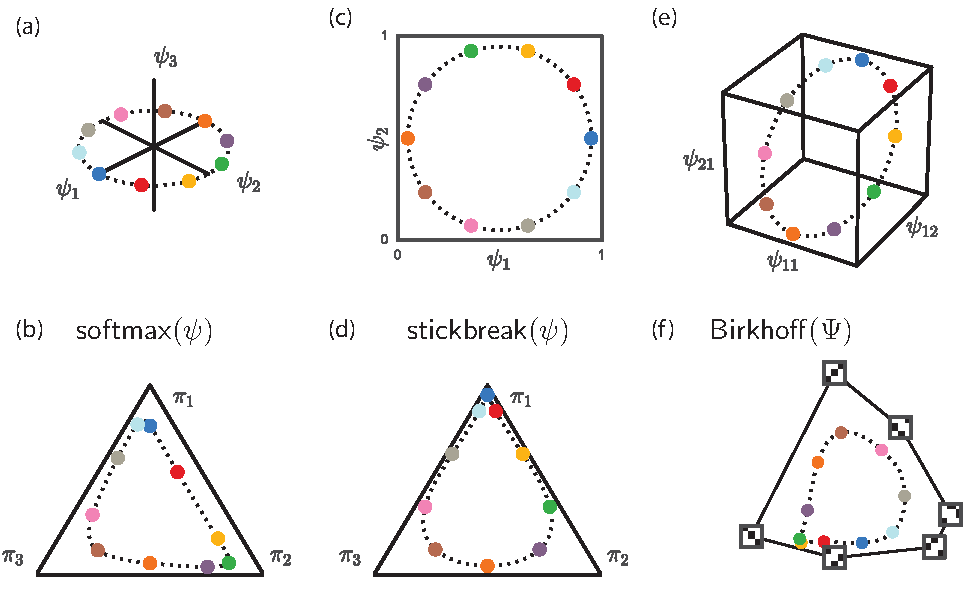
\includegraphics[width=5.in]{../figures/figure1.pdf} 
  \caption{
  }
\label{fig:transforms}
\end{figure*}



Recently, there have been a number of proposals for extending these
reparameterization tricks to high dimensional discrete
problems\footnote{Discrete inference is only problematic in the high
dimensional case, since in low dimensional problems we can enumerate
the possible values of~$x$ and compute the normalizing constant~$p(y)
= \sum_x p(y, x)$.} by relaxing them to analogous continuous
problems \citep{maddison2016concrete, jang2016categorical,
kusner2016gans}.  These approaches are based on the following
observation: if~$x \in \{0,1\}^k$ is a one-hot vector drawn from a
categorical distribution, then the support of~$p(x)$ is the set of
vertices of the~$k-1$ dimensional simplex.  Thus, we can represent the
distribution of~$x$ as an atomic density on the simplex.  Sampling~$x$
is equivalent to sampling this atomic measure. That is,
\begin{align}
  x &\sim \distCategorical( x \mid \theta) &\iff& & {\pi} &\sim p({\pi} \mid \theta) \nonumber \\
  & & & & x &\triangleq {\pi},
\end{align}
where~$p({\pi} \mid \theta)$ is a density on the simplex with atoms at
the~$k$ vertices.

Viewing~$x$ as a vertex of the simplex motivates a natural relaxation:
let us set~$x={\pi}$ as above, but 
rather than restricting~$p({\pi} \mid \theta)$ to be an atomic measure,
let it be a continuous density on the simplex. To be concrete, suppose
the density of~${\pi}$ is defined by the transformation,
\begin{align}
  \xi &\sim p(\xi), \\
  \psi & = g(\theta, \xi),  \quad g(\theta, \xi) = \log \theta + \xi,
\\
  {\pi} &=  \text{softmax}(\psi). \\
  \end{align}
The output~$x$ is now a point on the simplex, and the parameters~$\theta$ can
be optimized via stochastic gradient ascent with the reparameterization trick,
as discussed above.

In the aforementioned papers,~$p(\xi)$ is taken to be the Gumbel distribution.
This choice leads to a nicely interpretable model: adding
Gumbel noise and taking the argmax yields an exact sample from~$\theta$;
setting~$g$ to the softmax is a natural relaxation. Ultimately, however, this
is just a continuous relaxation of an atomic density to a continuous
density. 
\section{Methods}
\subsection{Alternative continuous relaxations}
\label{sub:alternative}
Here we introduce two alternative ways of conceiving a relaxed version of a discrete random variable that are also amenable for variational inference with Monte Carlo estimates of the gradient based on re-parameterization. However, unlike the Gumbel-Softmax, these relaxations enable extensions to more complex combinatorial objects; notably, permutations.

\subsubsection{Stick-breaking}
Consider the following alternative model for~${\pi}$:
\begin{align}
  \xi &\sim p(\xi) \\
  \psi & = g(\theta, \xi),  \\
  z &  = h(\psi), \;\; z\in[0,1]^{K-1}, \\ 
   {\pi} &=\mathcal{SB}(z), 
  \end{align}
 where the stick-breaking transformation $\mathcal{SB}(z_i)$ is defined by the assignment:
\begin{align} {\pi}_1 =z_1, \quad {\pi}_k = z_k \left(1- \sum_{j=1}^{k-1} {\pi}_j\right) \;\; \text{for } k=2, \ldots, K-1,  \quad {\pi}_K = 1- \sum_{j=1}^{K-1} {\pi}_j. 
\end{align}
In words: the noise distribution is transformed to $\psi$, which is latter constrained to belong to the unit hypercube through $z = h(\psi)$, assumed invertible. Then, we apply the stick-breaking transformation to $z$ to obtain a point $\pi$ on the simplex. $z_k$ can seen as the fraction of the remaining ``stick'' of probability mass assigned to~${\pi}_k$ \citep{linderman2015dependent}.


In this paper we focus on the choice $\psi_k \sim \distNormal(\mu_k, \eta_k^2) $ (i.e., $\xi\sim\distNormal(0,I), \theta = (\mu,\eta), g(\theta, \xi) = \mu + \eta \xi$), and $h(\cdot) = \sigma(\cdot /\tau)$ with $\sigma$ the logistic function. We name this the known as a logistic-normal stick-breaking transformation, which enjoys the following properties: i)the density of~${\pi}$ can be expressed in closed form as a function of~$\mu_k$ and~$\eta_k^2$, ii) the temperature~$\tau$ controls how
concentrated $p(\pi)$ is at the vertices of the simplex, iii) with appropriate choices of parameters, in the limit ~$\tau \to 0$ we can recover any categorial distribution, i.e., the density becomes concentrated on atoms at the~$K$ vertices, and iv) as ~$\tau \to \infty$, the density concentrates on a point in the interior of the simplex determined by the parameters, and for intermediate values, the density is
continuous on the simplex. 

Finally, we stress the above logistic-normal construction is not the only available: by taking $h(\cdot) $ the identity function we conceive two other reparameterizations, by letting $z$ have either a Kumaraswamy or Beta distribution on the unit interval. While the former is easily reparameterizable, the latter --- which leads to the generalized Dirichlet distribution on the simplex ---  is not, requiring an additional rejection sampling correction term on its implementation in variational inference.
%a Kumaraswamy distribution $z = \psi \sim \mathcal{KM}(a,b)$ and ii) by letting $z$ have a Beta distribution 
See the appendix for proofs of our claims and details on alternative constructions.


\subsubsection{Rounding}
This relaxation is based on the notion of partitioning the space into regions around central points. Specifically,  consider $M$ points $\mathcal{P}=\{p_m\}$ in $\mathbb{R}^K$ (e.g., but not restricted to, one-hot vectors). Now, given $\psi\in\mathbb{R}^K$ we define the rounding operator $$R^{P}(\psi)=\arg\min_{p_n} ||p_n-\psi||^2.$$
This operator partitions $R^K$ into $M$ different regions, the ``Voronoi'' cells with center $p_m$, 
\begin{equation}V^\mathcal{P}_{m}=\{\psi\in\mathbb{R}^K:\;||\psi-p_m||\leq ||\psi-p_i||,\forall i\}.\end{equation}
We might simply conceive a discrete distribution by the application of the above map to some continuous random variable. However, that is not differentiable. Then, instead we consider a map that pulls a point towards its rounded value, by taking a convex combination between both. Specifically, we consider the following sampling scheme:
\begin{align}
 \xi   &\sim p(\xi), \\
  \psi &= g(\theta, \xi), \\
  \pi &   =  \tau \psi + (1-\tau) R^\mathcal{P}(\psi) 
\end{align}

Clearly, in the temperature limit $\tau=0$ we recover a discrete distribution, but for intermediate values the obtained R.V. is still continuous. Then, this gives us a way to approximate discrete values by continuous ones, but differing with previous approaches in that the approximating values $z$ are not required to lie in the simplex, but anywhere. Notably, if $\psi$ is gaussian parameterized by its mean and standard deviation, by appropriate (limit) choices of parameters we can represent any arbitrary categorical distribution over one-hot vectors. This is shown in the appendix. 
 
\subsection{Continuous relaxations for distributions over permutations}
\label{sub:permutation}
To extend the above relaxations to also represent distributions over permutations we start by representing permutations $\sigma$ (now not the logistic function) of $N$ elements (i.e., the $N!$ biyections from $\{1,\ldots,N\}$ onto itself) as binary matrices $X\in \{0,1\}^ {N \times N}$, whose row and column sums equal one. Then, $X$ is like a one-hot vector but defined by a richer combinatorial structure. Notice that the rounding-based relaxation is available here, as the rounding operator can be casted as a matching problem, solved by the hungarian algorithm in $O(N^3)$ (see appendix). However, the stick-breaking equivalent for permutations is more involved: just as one-hot vectors are the vertices of the simplex, the Birkhoff-von Neumann
theorem states that permutation matrices are vertices of the convex
hull of doubly stochastic matrices. Then, an analogous relaxation is to consider~$X \approx {\Pi}$,
where ~${\Pi} \in [0,1]^{N \times N}$ is a doubly stochastic matrix,
i.e. the rows and columns both are positive and sum to one but entries are not necessarily zero or one. This set is known as the Birkhoff polytope, denoted ~$\cB_N$. Due to these constraints, ~$\cB_N$ lies within a~$(N-1)^2$ dimensional subspace of all $[0,1]^{N \times N}$ matrices.
 

We now derive an invertible and differentiable transformation,~$f: \reals^{(N-1) \times (N-1)} \to \cB_n$,
which can be used to define a density on~$\cB_N$, by extending the original stick-breaking transformation, with minor
modifications to accomodate the additional constraints of doubly stochastic
matrices. Imagine transforming a real-valued matrix~$\Psi \in \reals^{(N-1) \times (N-1)}$
into a doubly stochastic matrix,~${\Pi} \in [0,1]^{N \times N}$.
We work entry by entry, starting in the top left
and raster scanning left to right then top to bottom. Denote the~$(i,j)$-th entries
of~$\Psi$ and~${\Pi}$ by~$\psi_{ij}$ and~${\pi}_{ij}$, respectively.

The first entry is given by, ${\pi}_{11} = \sigma(\psi_{11})$.
As we work left to right in the first row, the ``remaining stick'' length
decreases as we add new entries. This reflects the row normalization constraints.
Thus,
\begin{align}
%  {\pi}_{1j} &= \sigma(\psi_{1j}) \prod_{k=1}^{j-1} (1-\sigma(\psi_{1k})) & &  \text{for } j=2, \ldots, n-1\\
  {\pi}_{1j} &= \sigma(\psi_{1j}) (1 - \sum_{k=1}^{j-1} {\pi}_{1k})  & &  \text{for } j=2, \ldots, n-1\\
  {\pi}_{1n} &= 1 - \sum_{k=1}^{n-1} {\pi}_{1k}
\end{align}
So far, this is exactly as above. However, the remaining rows must now
conform to both row- and column-constraints. That is,
\begin{align}
{\pi}_{ij} &\leq 1- \sum_{k=1}^{j-1} {\pi}_{ik} & & \text{(row sum)} \\
{\pi}_{ij} &\leq 1- \sum_{k=1}^{i-1} {\pi}_{kj} & & \text{(column sum)}.
\end{align}
Moreover, there is also a lower bound on~${\pi}_{ij}$. This entry must
claim enough of the stick such that what is leftover ``fits'' within the confines
imposed by subsequent column sums. That is, each column sum places an upper
bound on the amount that may be attributed to any subsequent entry. If the remaining
stick exceeds the sum of these upper bounds, the matrix will not be doubly stochastic.
Thus,
\begin{align}
\underbrace{1 - \sum_{k=1}^j \pi_{ik}}_{\text{remaining stick}}
&\leq \underbrace{\sum_{m=j+1}^n (1- \sum_{k=1}^{i-1} {\pi}_{km})}_{\text{remaining upper bounds}}.
\end{align}
Rearranging terms, we have,
\begin{align}
\pi_{ij} &\geq 1- \sum_{k=1}^{j-1} \pi_{ik} - \sum_{m=j+1}^n (1- \sum_{k=1}^{i-1} {\pi}_{km}) \\
&= 1 - n + j - \sum_{k=1}^{j-1} \pi_{ik}  +  \sum_{k=1}^{i-1} \sum_{m=j+1}^n {\pi}_{km}
\end{align}
Of course, this bound is only relevant if the right hand side is greater than zero.
Taken together,~${\pi}_{ij}$ is bounded by,
\begin{align}
\ell_{ij} &\leq
{\pi}_{ij}
\leq
u_{ij}
\\
\ell_{ij} &\triangleq \max \left \{0, \, 1 - n + j - \sum_{k=1}^{j-1} {\pi}_{ik}  +  \sum_{k=1}^{i-1} \sum_{m=j+1}^n {\pi}_{km} \right \}
\\
u_{ij} &\triangleq 
\min \left \{1- \sum_{k=1}^{j-1} {\pi}_{ik}, \,
1- \sum_{k=1}^{i-1} {\pi}_{kj} \right\}.
\end{align}
Thus, we define,
\begin{align}
  {\pi}_{ij} &= \ell_{ij} + \sigma(\psi_{ij}) (u_{ij} - \ell_{ij}).
\end{align}

The inverse transformation from~${\Pi}$ to $\Psi$ is analogous.
We start by computing~$\psi_{11}$ and then progressively compute
upper and lower bounds and set,
\begin{align}
\psi_{ij} &= \sigma^{-1} \left( \frac{{\pi}_{ij} - \ell_{ij}}{u_{ij} - \ell_{ij}} \right ).
\end{align}



 \subsection{Variational Inference}
To approximate an intractable posterior distribution over latent discrete or permutation valued variables we choose the best (in the KL sense) among the parametric families that we have described. Now we describe the most relevant details.

\subsubsection{From continuum to discrete}
Doing a continuous relaxation requires re-thinking the objective. As in \cite{maddison2016concrete}, we maximize a relaxed ELBO, for which we need to specify a new continuous prior $p(\pi)$ over the latents. This prior should be peaked around the discrete points for which inference is required, so we can conceive the original discrete ELBO through a limiting process. Good, peaked priors are necessary as the likelihood $p(y|\pi)$ could be large for points that have nothing to do with the original problem, leading to nonsensical solutions. There is a trade-off, though: priors that are too peaked will lead to multiple local maxima of the ELBO, preventing optimizers from achieving the right solution.Then, for optimal performance the prior has to be treated as a hyperparameter. Here, for one-hot vectors we considered mixture of gaussians around each point (parameterized by the variance), and for permutations, we considered the product of $N$ one-dimensional mixture of gaussians around zero and one. Although this prior puts significant mass on points that are not interesting (e.g. (1,1,\ldots, 1)), at least it penalizes $\pi$ that are too away from ~$\cB_N$.


\subsubsection{Estimating the ELBO}
Notice in all the relaxations discussed here, $\pi = F(\psi)$ where $F$ is a differentiable and invertible function  (see the appendix for details). Therefore, by the change of variable theorem and the law of the unconscious statistician:
$$ \E_{p(\xi)} \left[- \log q(F(g(\theta, \xi)); \theta) \right] = Entropy(\psi;\theta)+E_{p(\xi)}\left[\log | DF(g(\theta, \xi))|\right],$$
where the term inside of the expectation is the (log) Jacobian of $F$ evaluated at $\psi = f(\theta,\xi)$. Then, if this Jacobian and the entropy of $\psi$ are available we can consider an unbiased estimator for the ELBO:

$$\hat{\cL}(\theta) = Entropy(\psi) +  \frac{1}{L}\sum_{l=1}^L \left[ \log p(y,  g(\theta, \xi_l) ) +  \log |DF(g(\theta, \xi_l)|\right].$$

For example, for rounding, $F$ is piecewise linear \footnote{the set of discontinuities has Lebesgue measure zero so we can still apply the change of variables theorem.} and $\log | DF(g(\theta, \xi)) |= K\log \tau$. Also, if $\psi$ is gaussian its entropy is given by $K\log(\eta^2 2\pi e  )/2$.


\subsubsection{Constraining the parameters}
For rounding-based permutation inference, we found that an efficient way of avoiding evaluation of the likelihood in non-relevant points is to constrain $\mu$ to belong to ~$\cB_N$. This can be done applying Sinkhorn propagation, i.e., successively normalizing the rows and columns of the matrix $\mu$. The resulting $\mu$ is guaranteed to converge to a point in ~$\cB_N$, which will remain close if $\eta$ is small.
\section{Results}
Here we summarize our main results. See the appendix for implementation details.
\subsection{Variational Autoencoders (VAE) with categorical latent variables}
We first demonstrate that our proposed relaxations are sensible for categorical random variables, and can be efficiently implemented within the current dominant computational frameworks. We considered the density estimation task on MNIST digits, as in \cite{maddison2016concrete, jang2016categorical}, where observed digits are thought as reconstructed from a latent discrete code. We used the continuous ELBO for training, and evaluated performance based on the marginal likelihood, estimated through the multi-sample variational objective of the discretized model (via rounding the samples $\pi$) with $m=1000$. We trained our models using ADAM in Tensorflow and compared agains the method of \cite{jang2016categorical}, finding similar results (Table 1). Also, better results were obtained with rounding. Our results suggest our methods provide a viable alternative to the Gumbel-Softmax. In figure \ref{fig:VAE} we show some reconstructed images using the different approaches.


\begin{table}[t]
  \caption{Summary of results in VAE}
  \label{sample-table}
  \centering
  \begin{tabular}{llll}

    %\multicolumn{4}{Method}                   \\
    \midrule

    & Gumbel-Softmax    & Rounding & Stick-breaking\\
    \cmidrule{2-4}
    - $\log p(x)$ & 113.9  & $\sim$106.9  & 12    \\
        \bottomrule
  \end{tabular}
\end{table}


 \subsection{Synthetic matching experiments}
To assess the quality of our approximations for distributions over permutations, we considered a toy problem where $N=6$ points in $\mathbb{R}^2$ where normally sampled around other fixed $N=6$ centers, with varying standard deviation $\sigma$. This naturally induces a posterior distribution of assignments between samples and the centers they come from \footnote{think of this as a variation of the mixture of gaussians models, where now each center is associated with a unique sample}, and as $N!=720$ is moderate, this posterior can be computed exactly by enumeration. We measured discrepancy through the Battacharya distance (BD) between true histogram and the histogram of the approximated posterior constructed by sampling from $q(\pi)$ and 'rounding' to the nearest permutation using the Hungarian algorithm. We found our methods provide reasonable fit to the true posterior, allowing to represent more complex distributions over permutations than, e.g., simple Mallows distribution around the MAP estimate. In figure \ref{fig:synthetic}\begin{figure*}[t] we show examples of true posteriors (ranked) and their approximations, and quantify the discrepancies by the distribution of the BD.
  \centering
  \includegraphics[width=1.0\textwidth]{../figures/figure5.pdf} 
  \caption{}
\label{fig:VAE}
\end{figure*}

\label{sub:synthetic}


\begin{figure*}[t]
  \centering
  \includegraphics[width=5.in]{../figures/figure4.pdf} 
  \caption{Examples of true and reconstructed digits from their corresponding random codes using with $N=20$ categorical variables with $K=10$ possible values. In any case 
  }
\label{fig:synthetic}
\end{figure*}

\label{sub:vae}

\subsection{Hierarchical permutation inference}
\label{sub:synth_celegans}



\bibliography{refs}
\bibliographystyle{abbrvnat}

\appendix
\section{Limit analysis}
\subsection{Stick-breaking}
Here we state and prove that for all the stick-breaking based distributions in the simplex we consider here; based on the Logistic-gaussian, Kumaraswamy, and Beta distributions, we can arrive to any point in the interior of the simple or any categorical distribution as limiting cases (in $\tau$). First, we need some lemmas.


\textbf{Lemma 1.}  The following statements are true:
\begin{enumerate} \item the degenerate case where  $z_k$ is deterministic leads to $\pi\sim \delta(\tilde{\pi})$  (i.e, single atom in the point $\tilde{\pi}$). Also, if $z_k$ can be any in $(0,1)$ then any deterministic $\pi$ in the interior of the simplex can be realized.
\item the degenerate case where  $z_k$ are Bernoulli with parameter $p_k(\theta) \in (0,1)$ leads to $\pi$ having an atomic distribution with atoms in the vertices of $\Delta^{k-1}$; i.e, $\pi$ is categorical. We have the following expression for the probabilities of the atoms $\pi_k=1$ (one hot vectors):
\begin{align}
\label{eq:onehotprob}
P(\pi_k =1)&= \prod_{i=1}^{k-1} (1-p_i(\theta)) p_k(\theta)  \;\; \text{for } k=2, \ldots, K-1, \quad P(\pi_K =1) = \prod_{i=1}^{K-1} (1-p_i(\theta)).
\end{align}

Moreover, if for each index $k$ any parameter of the Bernoulli variable $z_k$ can be realized through appropriate choice of $\theta$, then any categorical distribution can be realized.

\end{enumerate}
\textit{Proof}: (a) both claims are obvious and come from the invertibility of the function $\mathcal{SB} \circ h (\cdot)$. (b) the formulae for $P(\pi_k =1)$ comes from expressing the event $\pi_k=1$ equivalently as $\pi_k=1,\pi_i=0, i<k$ and then, conditioning backwards successively. The second statement comes from the following expression, which easily follows  from \eqref{eq:onehotprob}:
$$ p_k(\theta)=\frac{P(\pi_k =1)}{P(\pi_{k-1} =1)}\frac{p_{k-1}(\theta)}{1-p_{k-1}(\theta)},\quad k =1,\ldots, K-1.$$
The recursive nature of the above equation gives a recipe to iteratively determine the required $p_k(\theta)$, given  $P(\pi_k =1), P(\pi_{k-1} =1)$ and the already computed $p_{k-1}(\theta)$.


Now we can state our results:

\textbf{Lemma 2.} If $z=\sigma(\psi),\psi\sim\mathcal{N}(\mu,\eta^2)$, then
\begin{enumerate} \item the  limit $\eta\rightarrow 0$ and $\mu$ fixed leads to the deterministic $z=\sigma(\mu)$. 
\item the limit $\mu\rightarrow \infty, \eta^2=\mu/K$ with K constant leads to $z\sim \text{Bernoulli}(\Phi(K))$, with $\Phi(\cdot)$ denoting the standard normal cdf.
\end{enumerate} In both cases the convergence is in distribution 

\textit{Proof}. The first convergence is obvious. To see the second, let's index $\mu_n$ and  study the cdf $F$ of $z_n$ on the interval (0,1) (it evaluates zero below zero and one above one).
\begin{align}F_{z_n}(x)&= P(\sigma(\psi_n)<x) \\
&=P(\psi_n< \sigma^{-1}(x))\\
&=P(\mu_n +\mu_n/K\xi <\sigma^{-1}(x)),\\\
&= P( \xi <\sigma^{-1}(x)K/\mu_n - K)\\
&= \Phi( \sigma^{-1}(x)K/\mu_n - K) 
\end{align}

Therefore, by continuity of $\Phi$ we obtain $F_{\Psi_n}(x)\rightarrow \Phi(-K)$ for all points $x\in(0,1)$. On the other hand, the cdf of a bernoulli random $F$ variable is given by  a step function that abruptly changes at zero, from zero to $1-p$, and at one, from $1-p$ to 1. As convergence occurs at all continuity points (the interval $(0,1)$), we conclude (recall, $1-p= \Phi(-K)\rightarrow \Phi(K)=p$). Notice that the above representation only allows  to converge to $p>0.5$, as $K$ has to be positive. This can be fixed by choosing sequence with negative $\mu$ instead.

\textbf{Lemma 3.} If $z=\mathcal{K}(a,b)$: \begin{enumerate}
\item in the limit $a,b \rightarrow $  we converge to deterministc $p$, provided that $p=bB\left(1+\frac{1}{a},b\right)$ along the limiting sequence.
\item In the limit $a,b\rightarrow 0$ we obtain convergence to a Bernoulli random variable with parameter $p$, provided the same condition involving $p,a,b$ holds. 
\end{enumerate}
In both cases convergence is in probability.
\textit{Proof}: A proof can be found in \cite{mitnik2013kumar}

\textbf{Lemma 4.} If $z=Beta(a,b)$: \begin{enumerate}
\item in the limit $a,b \rightarrow \infty $  we converge to deterministc $p$, provided that $p=bB\left(1+\frac{1}{a},b\right)$ along the limiting sequence.
\item In the limit $a,b\rightarrow 0$ we obtain convergence to a Bernoulli random variable with parameter $p$, provided the same condition involving $p,a,b$ holds. 
\end{enumerate}
In both cases convergence is in distribution.

\textbf{Proposition.} In all the discussed cases of re-parameterizations of the simplex via stick-breaking, arbitrary categorical distributions can be obtained in the low-temperature limit. Also, in the high-temperature convergence is to certain point(s) in the interior of the simplex.

\textit{Proof}: Consider each distribution separately
\begin{enumerate}
\item For the logistic-normal re-parameterization $z_k = \sigma\left( \frac{\mu_k+\eta_k\xi}{\tau}\right)$, in the low temperature case use Lemma 2 (b) by the always available representation  $K= \frac{\mu}{\eta^2}$and conclude by Lemma 1(b). In the high temperature case convergence is to the point $\pi = \mathcal{SB}(0.5,0.5,\ldots, 0.5)$.
\item For Kumaraswamy $z_k=\mathcal{K}(a_k,b_k)$ the argument is similar, but here the temperature can only be defined implicitly through sequences of parameters $(a_k,b_k)$ converging to either $\infty$ or 0 along a sequence with fixed $p_k=b_kB\left(1+\frac{1}{a_k},b_k\right)$. Then in the low temperature case we conclude by Lemma 3(b) and Lemma 1(b). In the hig-temperature case we converge to the point $SB(p_1,\ldots p_{k-1}$
\item For the Beta $z_k\sim Beta(\frac{a_k}{\tau},\frac{b_k}{\tau})$ low-temperature leads to convergence to $z_k$ Bernoulli with parameter $a_k/(a_k+b_k)$ and we conclude from Lemma 4(b) and Lemma 1(b). For high temperatures, convergence is to the point $\mathcal{SB}(a_k/(a_k+b_k),\ldots,a_{k-1}/(a_{k-1}+b_{k-1}))$.  \end{enumerate}


\subsection{Rounding}
Here we have two extremes: at $\tau =1$ we obtain a continuous distribution in the space (here, gaussian). If $\tau=0$ the resulting distribution has only atoms in the one-hot vectors $p_n$, in this proof assumed to be the one-hot vectors. We show that in this case it is possible to represent any arbitrary categorical distribution through a judicious choice of the parameters.


\textbf{Proposition:} In the zero temperature case, i.e., $\pi  = R^\mathcal{P}(\psi)$ it is possible to represent any arbitrary distribution i.e, for any $\alpha$ in the $N-1$ simplex there exists gaussian parameters $(\mu, \eta)$ so that   $P(\pi = p_n)  = \alpha_n$. Points inside the simplex are realized directly, while distributions with some $\alpha_k=0$ are realized through a limiting process in the parameters.

\textit{Proof:} First set $\eta_n=1$. By representing $\psi = \mu + \xi$ where $\xi\sim\distNormal(0, I)$ we see that
$$\alpha_n = P(R^\mathcal{P}(\mu + \xi) = p_n ) = P(\mu + \xi \in V^\mathcal{P}_{n}) = P(\xi \in V^\mathcal{P}_{n} - \mu) =  \int_{V^\mathcal{P}_{n} - \mu} \frac{1}{(2\pi)^\frac{N}{2}}e^{-\frac{||x||^2}{2}} dx.$$
Three conclusions are drawn from the above: first, we see that probabilities are ultimately gaussian integrals over a new partition, a translation of the Voronoi regions $V^\mathcal{P}_{n}$. Second,
the map $(\mu_1,\ldots,  \mu_n)\xrightarrow{m} (\alpha_1,\ldots, \alpha_n)$ is continuous by virtue of the dominated convergence theorem \cite{browder2012mathematical}: indeed, if $\mu_i\rightarrow \mu$ then $(\alpha^i_1,\ldots, \alpha^i_n) \rightarrow (\alpha_1,\ldots, \alpha_n)$, as the $\alpha^i_n$ are integrals that can be expressed using indicator functions in the integrands (which are all bounded by the integrable gaussian density), and as pointwise convergence of the indicators holds because of the continuity of the translation operator $f_\mu(\cdot) = \cdot + \mu$. Third, for each $q\in(0,1)$ it is possible to choose $\mu$ so that $\alpha_n =q$ and $\alpha_m = (1-q)/(n-1)$. Indeed, by moving $\mu_n$ between $-\infty$ and $\infty$ while keeping the other $\mu_k$ fixed then $V^\mathcal{P}_{n} - \mu$ fluctuates between the empty set ($\alpha_n =0$) and the entire space ($\alpha_n=1$). Therefore, by the continuity of $m$ and the intermediate value theorem, every value in $\alpha_n\in (0,1)$ is realized, and by symmetry the other $\alpha_k$ occupy the remaining mass uniformly. 

To conclude, we use the fact that the image of a convex set through a continuous function is also convex \cite{Rockafellar70}. We also showed that for each tolerance $\epsilon$ the image of $m$ contains these $\epsilon$-one-hot vectors: that is, the points with $(1-\epsilon)$ in one coordinate and $\epsilon/ (n-1)$ in the rest. Then, given a point in the interior of the simplex choose $\epsilon$ small enough so it is in the convex hull of the $\epsilon$-one vectors. Then, by the above theorem there must be a pre-image $\mu$ that realizes this point.

For $\alpha$ with zero entries the above arguments has to be extended to permit a limit process where $\mu$ goes to either infinity or infinity. It is easy to see that by that extension it is possible to represent any $\alpha$ in the border of the simplex.

\section{Deriving  the approximation for the ELBO}
Here we show that $$\E_{p(\xi)} \left[- \log q(F(g(\theta, \xi)); \theta) \right] = Entropy(\psi; \theta)+E_{p(\xi)}\left[\log | DF(g(\theta, \xi))|\right].$$
Indeed, first, by the `Law of the Unconscious Statistician' we have:
 $$\E_{p(\xi)} \left[- \log q(F(g(\theta, \xi)); \theta) \right] = \E_{p(\psi;\theta)} \left[- \log q(F(\psi); \theta) \right]. $$
Now, by the change of variable theorem and derivative and determinant inversion rules, we obtain:\begin{align}
q(F(\psi); \theta) & = p(F^{-1}(\pi) ;\theta)  |DF ^{-1}(\pi) | \\
 & = p(\psi;\theta) | DF (\psi) | ^{-1}.
 \end{align}
 To conclude we use once more the Law of the Unconscious Statistician:
 \begin{align}
 \E_{p(\xi)} \left[- \log q(F(g(\theta, \xi)); \theta) \right]  &= \E_{p(\psi;\theta)}\left[ - \log p(\psi;\theta)\right] +   \E_{p(\psi;\theta)}\left[\log | DF(\psi)|\right] \\
 &= Entropy(\psi; \theta)+E_{p(\xi)}\left[\log | DF(g(\theta, \xi))|\right].\end{align}
 
 Notice $R^Z$ is a piecewise constant function, as maps each $V^\mathcal{P}_{m}$ to $p_m$

Notice that these bounds only depend on values of~${\Pi}$ that
have already been computed; i.e., those that are above or to the left of
the~$(i,j)$-th entry. Thus, the transformation from~$\Psi$ to~${\Pi}$
is feed-forward according to this ordering.  Consequently, the
Jacobian of the inverse transformation,~$\mathrm{d}\Psi / \mathrm{d} \Pi$,
is lower triangular, and its determinant is the product of its diagonal,
\begin{align}
\left| \frac{\mathrm{d} \Psi } {\mathrm{d} \Pi} \right|
&= \prod_{i=1}^{n-1} \prod_{j=1}^{n-1} \frac{\partial \psi_{ij} }{\partial {\pi}_{ij}} \\
&= \prod_{i=1}^{n-1} \prod_{j=1}^{n-1} \frac{\partial}{\partial {\pi}_{ij}}
\sigma^{-1} \left( \frac{{\pi}_{ij} - \ell_{ij}}{u_{ij} - \ell_{ij}} \right ) \\
&= \prod_{i=1}^{n-1} \prod_{j=1}^{n-1}
\left( \frac{1}{u_{ij} - \ell_{ij}} \right )
\left( \frac{u_{ij} - \ell_{ij}}{{\pi}_{ij} - \ell_{ij}} \right )
\left( \frac{u_{ij} - \ell_{ij}}{u_{ij} - {\pi}_{ij}} \right ) \\
&= \prod_{i=1}^{n-1} \prod_{j=1}^{n-1}
\frac{u_{ij} - \ell_{ij}}{({\pi}_{ij} - \ell_{ij}) (u_{ij} - {\pi}_{ij})}
\end{align}

With these two ingredients, we can write the density of~${\Pi}$,
\begin{align}
  \text{vec} (\Psi) &\sim \distNormal(\mu, \diag(\eta^2))
  \\
  {\Pi} &= f(\Psi) \\
  \implies
  p(\Pi \mid \mu, \diag(\eta^2)) &= \left|\frac{\mathrm{d} \Psi }{\mathrm{d} {\Pi}} \right|
  \distNormal(f^{-1}({\Pi}) \mid \mu, \diag(\eta^2))
\end{align}

Given the density and a differentiable mapping we can perform
variational inference with stochastic optimization of the ELBO.
We define a distribution over doubly stochastic matrices as a
reparameterization of a multivariate Gaussian distribution
over~$\Psi$. We can estimate gradients via the reparameterization
trick.

It is important to note that the transformation is only piecewise
continuous: the function is not differentiable at the points where
the bounds change; for example, when changing~$\Psi$ causes the
active upper bound to switch from the row to the column constraint
or vice versa.  I think we can argue that these discontinuities
will not have a severe effect on our stochastic gradient algorithm.




\end{document}